\chapter{Implementations}
\label{chpt:implementations}

\epigraph{You are not expected to understand this}{\textit{John Lions, Lions' Commentary on UNIX 6th Edition, with Source Code}}
%%%%%%%%%%%%%%%%%%%%%%%%%%%%%%%%%%%%%%%%%%%%%%%%%%%%%%%%%



%%%%%%%%%%%%%%%%%%%%%%%%%%%%%%%%%%%%%%%%%%%%%%%%%%%%%
%%% intro
\section{Not another introduction!}
\begin{comment}
Classical computers are ubiquitous in today's society. They are present in nearly every electronic device, from embedded microcontrollers in washing machines and fridges, through microprocessors in mobile phones and computers, all the way to large scale servers and mainframes controlling critical infrastructure and powering the internet. 

Three features of computers make this possible: the ability to pack millions of transistors into a single silicon die; the extremely small cost of doing it; and the existence of software that abstract away implementation details.
\end{comment}

The vast majority of tasks facing modern programmers require little or no knowledge of how computers really work. There is a wealth of programming languages and development tools which remove implementation details and allow the engineer to focus on the important aspects of the task at hand.

However, due to the lack of large scale quantum computers, complex software stacks and quantum development environments which hide implementation details simply do not exist. We therefore consider it necessary to understand at least the basics of how quantum computers might work.

The section is arranged as follows. We begin with a historical overview of classical computers, and a brief description of classical architectures. We then contrast this with the multitude of current approaches to quantum computation. We look at quantum computer hardware and the physical systems which represent qubits and implement quantum operations. 

We then discuss how the languages we've included in the guide can be turned into programs that run on quantum hardware. We conclude by comparing this process with the steps needed to control a classical computer.
\begin{comment}
Finally we discuss possible architectures of future large scale quantum computers.
\end{comment}

%%%%%%%%%%%%%%%%%%%%%%%%%%%%%%%%%%%%%%%%%%%%%%%%%%%%%%%%
% classical computers
\subsection{Classical hardware}
\label{sec:classicalquantumhardware}

In the past there have been many different approaches to classical computation. Some devices such as the abacus or slide rule are simple mechanical devices that are operated manually, but which speed up certain operations (e.g. arithmetic). Charles Babbage's difference engine uses a complicated system of cogs and gears to perform more general purpose operations. In an analog computer, voltages and currents are used to represent variables. Analog computers can solve differential equations and model physical systems.

During the middle and latter half of the 20\textsuperscript{th} century, there was a substantial move to replace all these methods with general purpose computers based on digital electronics. Digital electronics uses two voltage levels, for example \SI{0}{\volt} and \SI{5}{\volt}, to encode a bit. Bits can be manipulated using digital logic circuits. One of the first digital computers was the Electronic Numerical Integrator and Computer (ENIAC), which was completed in 1945. ENIAC was re-programmable and Turing-complete. However, the thousands of valves required made it bulky and expensive. 

The large scale nature of these systems made it necessary to think carefully about the architecture of large scale computers. The Electronic Discrete Variable Automatic Computer (EDVAC), which followed the ENIAC, prompted Von Neumann to write a document outlining the high level operation of general operation of digital computers \cite{vonneumann1993first}. His proposed architecture for a digital computer became known as the Von Neumann architecture. It outlines the type of resouces that a classical computer would need, and how they would be connected together.

Following the invention of the transistor in the late 1940s, it became much easier to realise basic operations such as AND and OR gates, which could be used as the basis for digital computers. Transistors are much smaller, more reliable and more robust that valves. However, it was the invention of the integrated circuit in the 1950s which really kick started the digital computing revolution \cite{kilby1976invention}. Integrated circuits make it possible to squash electronics onto silicon chips, which dramatically reduces both the size of the resulting electronics and the time required to assemble circuits, which would previously have been hand soldered. The first computer to use integrated circuits was the IBM 360 in 1964 \cite{ibm360record}. 

These computers were bulky and expensive, comprising of a large mainframe, and small input output devices called terminals, which have a keyboard and a screen that allow users to interact with the mainframe. However, as discussed in \autoref{chpt:intro}, computers have become smaller and smaller, culminating in laptops, tablets and smartphones which can outperform the mainframes of the 60s.

As a result of all this success, microelectronics is the only classical computing `platform'. Normally, microprocessors share the following common features:
\begin{itemize}
    \item{\textbf{Memory}: processors require blocks of internal or external random access memory (\textbf{RAM}) which can store data and programs.}
    \item{\textbf{Working registers}: these are used for performing operations on data, e.g. the processor moves data to the working registers to perform an operation such as addition}
    \item{\textbf{Arithmetic and logic unit (ALU)} and \textbf{floating point unit (FPU)}: for performing logical and mathematical operations.}
    \item{ \textbf{Control}: this manages all the resources of the processor. The control unit is responsible for reading, decoding and executing instructions. Instructions are the simplest blocks of processing a classical computer can do}
    \item{\textbf{Buses}: shared data lines which can be used to move data between different parts of the processor.}
    \item{\textbf{Input/output}: for interacting with external devices. For example, a modern processor in a laptop will connect to external memory (e.g. more RAM, a hard drive), dedicated graphics hardware, a keyboard and display, etc.}
\end{itemize}

The classical architecture of a microprocessor is the precise manner in which the above building blocks are implemented and connected together. \autoref{fig:cpuHarvArch} shows the Harvard architecture, where the memory for storing data is different to the memory used for storing the program. The von Neumann architecture (\autoref{fig:cpuVonneuman}) discussed above uses the same physical memory for both the data and the program. Other architectural decisions include the width of the memory (e.g. 32 bit or 64 bit), the size of the instruction set (Intel chips for computers use large instruction sets; ARM devices for embedded applications have smaller instruction sets), and input/output capabilities (Intel chips might interact with graphics cards, whereas a Microchip microcontrollers might have a motor driver for use in automation applications.)

\begin{figure}[H]
    \centering
    \includegraphics[width=0.8\textwidth]{figures/impl/Harvard_architecture.png}
    \caption{Harvard Architecture}
    \label{fig:cpuHarvArch}
\end{figure}

\begin{figure}[H]
\centering
\includegraphics[width=0.8\textwidth]{figures/impl/Von_neumann_architecutre.png}
\caption{Von Neuman}
\label{fig:cpuVonneuman}
\end{figure}

\subsection{Quantum hardware}

In contrast with classical computers, there are comparatively few components in a quantum computer:

\begin{itemize}
    \item{\textbf{Qubits}: fundamental units of quantum information which can be in the state 0 or 1 like bits, but can also be in a superposition state. It must be possible to initialise a qubit in at least the zero state.}
    \item{\textbf{Quantum gates}: these are quantum operations which change the state of qubits. Typically gates which act on one or two qubits are considered most important, because it is possible to build up other more general gates from just these types}
    \item{\textbf{Measurements}: quantum computers must contain a system for making measurements on qubits -- these always return either 0 or 1 and allow useful information to be extracted from the computer} 
\end{itemize}

There are also speculative requirements such as quantum memory that may eventually be needed. It is unclear at this stage exactly what components a large scale quantum computer will contain.

More stuff here plz.

There is currently no large scale quantum computer.

%%%%%%%%%%%%%%%%%%%%%%%%%%%%%%%%%%%%%%%%%%%%%%%%%%%%%%%%%
\subsubsection{Cloud based quantum computing}

Cloud based quantum computing is likely to remain the most realistic method of getting access to a quantum computer in the near future. Just like the early years of digital computing, access to a computer was only possible through the introduction of mainframes and terminals, due to the huge cost and space needed for current small scale quantum devices this is the most feasible approach. However, with access to the internet the 'mainframe computer' can be accessed from all over the world. 

\begin{comment}
\begin{figure}[H]
    \centering
    \includegraphics[width=0.5\textwidth]{Forest_structure.PNG}
    \caption{The structure of Forest. Figure taken from \cite{Rigetti2016} - we will replace this with a general version for all languages and chips}
    \label{fig:rigettifullstack}
\end{figure}
\end{comment}

pyQuil, Qiskit and Project Q are all cloud based quantum libraries, with the appropriate access instructions for each given in \autoref{chpt:quantumsoftware}, code can be ran on the companies devices. Executing code on the quantum devices costs credits which you can apply for on the IBM Qiskit website.  

Like all of the languages discussed in this guide they use the approach of focusing on short-term quantum devices and adopt the dedicated quantum processor and classical processor structure.



\section{Quantum platforms}

The over-arching physical realisation of the components for quantum computers can be separated into two parts: the architecture and the platform. The platform is the physical system that is used to build the computer. Examples include photonics, trapped ions, semi-conductor qubits, and super-conducting qubits.

Quantum architecture has a more restricted meaning than in the classical case, due to the lack of large scale structure in a quantum computer. It refers to the manner in which the physical platform is used to realise qubits and gates. This is analogous to the different ways transistors can be used to create logic gates, for example transistor-transistor logic (TTL) or complementary metal oxide semiconductor (CMOS). As a result, the quantum architectures and platforms are not completely independent; some physical systems are much better suited to specific architectures. For example, the gate model is a natural choice when using trapped ions or superconducting qubits, whereas photonics is much better suited to one way quantum computing.

There are two distinct types of qubits, stationary (e.g. Trapped ions or superconducting qubits) or flying qubits (photons). Here we will only discuss trapped ions and photons as we believe these systems are the easiest to visualise conceptually. 

A good way to think of a quantum computer is a very large, noisy machine which is incredibly sensitive to its environment. The main difficulty is just trying to control it; most of the resources are used are for error correction, keeping the whole thing coherent. The remaining small part of the machine is for the information processing. 

\begin{comment}
\begin{itemize}
    \item intro what they are \& stability
    \item speed and gates
    \item scheme for impl
\end{itemize}
\end{comment}

%%%%%%%%%%%%%%%%%%%%%%%%%%%%%%%%%%%%%%%%5555
\subsection{Trapped Ions}

Trapped ions are a relatively stable physical system, which is a desirable feature for a quantum computer. Electric fields are used to trap the ions and individual ions can be shuttled around by changing the voltage in the direction you want the ion to move. This enables a great deal of control over the dynamics of the ions.

The quantum gates are performed on the qubits using either microwaves which use atomic transitions or optical pulses for electronic transitions. Microwave gates are appealing as it opens the possibility of addressing multiple qubits at once. 

\begin{comment} This will be necessary when taking into account error correction as one logical X operation could correspond to 100s or 1000s of X operations on physical qubits to produce one logical X. 
\end{comment}

The \cite{lekitsch2015blueprint} blueprint is a scheme which uses a modular approach of packing tiles shown in \autoref{fig:iontrap} on a 2D surface. Each tile contains the following: one ion, a dedicated loading zone, an entangling zone which interlinks ions on adjacent tiles and a detection zone for readout. Entangling gates or operations are performed by bringing two qubits close together. 

\begin{figure}[H]
    \centering
    \includegraphics[width=0.45\textwidth]{figures/impl/iontrap.png}
    \caption{An X-junction ion trap array with different trapping regions for entanglement, loading and detection, taken from \cite{lekitsch2015blueprint}.}
    \label{fig:iontrap}
\end{figure}

\begin{comment}
Another similar approach would see ion-trap modules each containing a small number of qubits linked together with fibre photonic connections to transmit the quantum information between modules. This approach could also be scaled-up as trapping ions in small numbers has been demonstrated with high-fidelity operations \cite{Harty2016}.

where the qubits where information can be lost after a certain amount of time. The clock speed determines the rate of calculations performed, and hence the gates applied must occur in this time period before the information is lost.   
\end{comment}

%%%%%%%%%%%%%%%%%%%%%%%%%%%%%%%%%%%%%%%%%%%
\subsection{Superconducting qubits}

Superconducting qubits (also called flux or charge qubits) are currently being worked on the most by private companies. The platform requires very cold temperatures in order to reach the superconducting regime. This will be problematic for future larger devices which will require larger and more expensive cryostats. Eventually we wont be able to fit the device inside a single cryostat placing a limit on the capacity of a single chip. It is generally believed within the field that cryostats will have to be interconnected for large scale computing which presents its own technical challenges. The cryogenic temperatures also pose a problem for control electronics\footnote{It is not well understood how traditional electronics behaves at cryogenic temperatures}.   
A potential benefit to overcoming these engineering challenges is that the platform is very quick which is indicative of a high clock speed in future devices. \autoref{fig:superconducting} is a 2 qubit superconducting chip, the gold wires around the device are for the control electronics for performing gates and measurement readout. 

\begin{figure}[H]
    \centering
    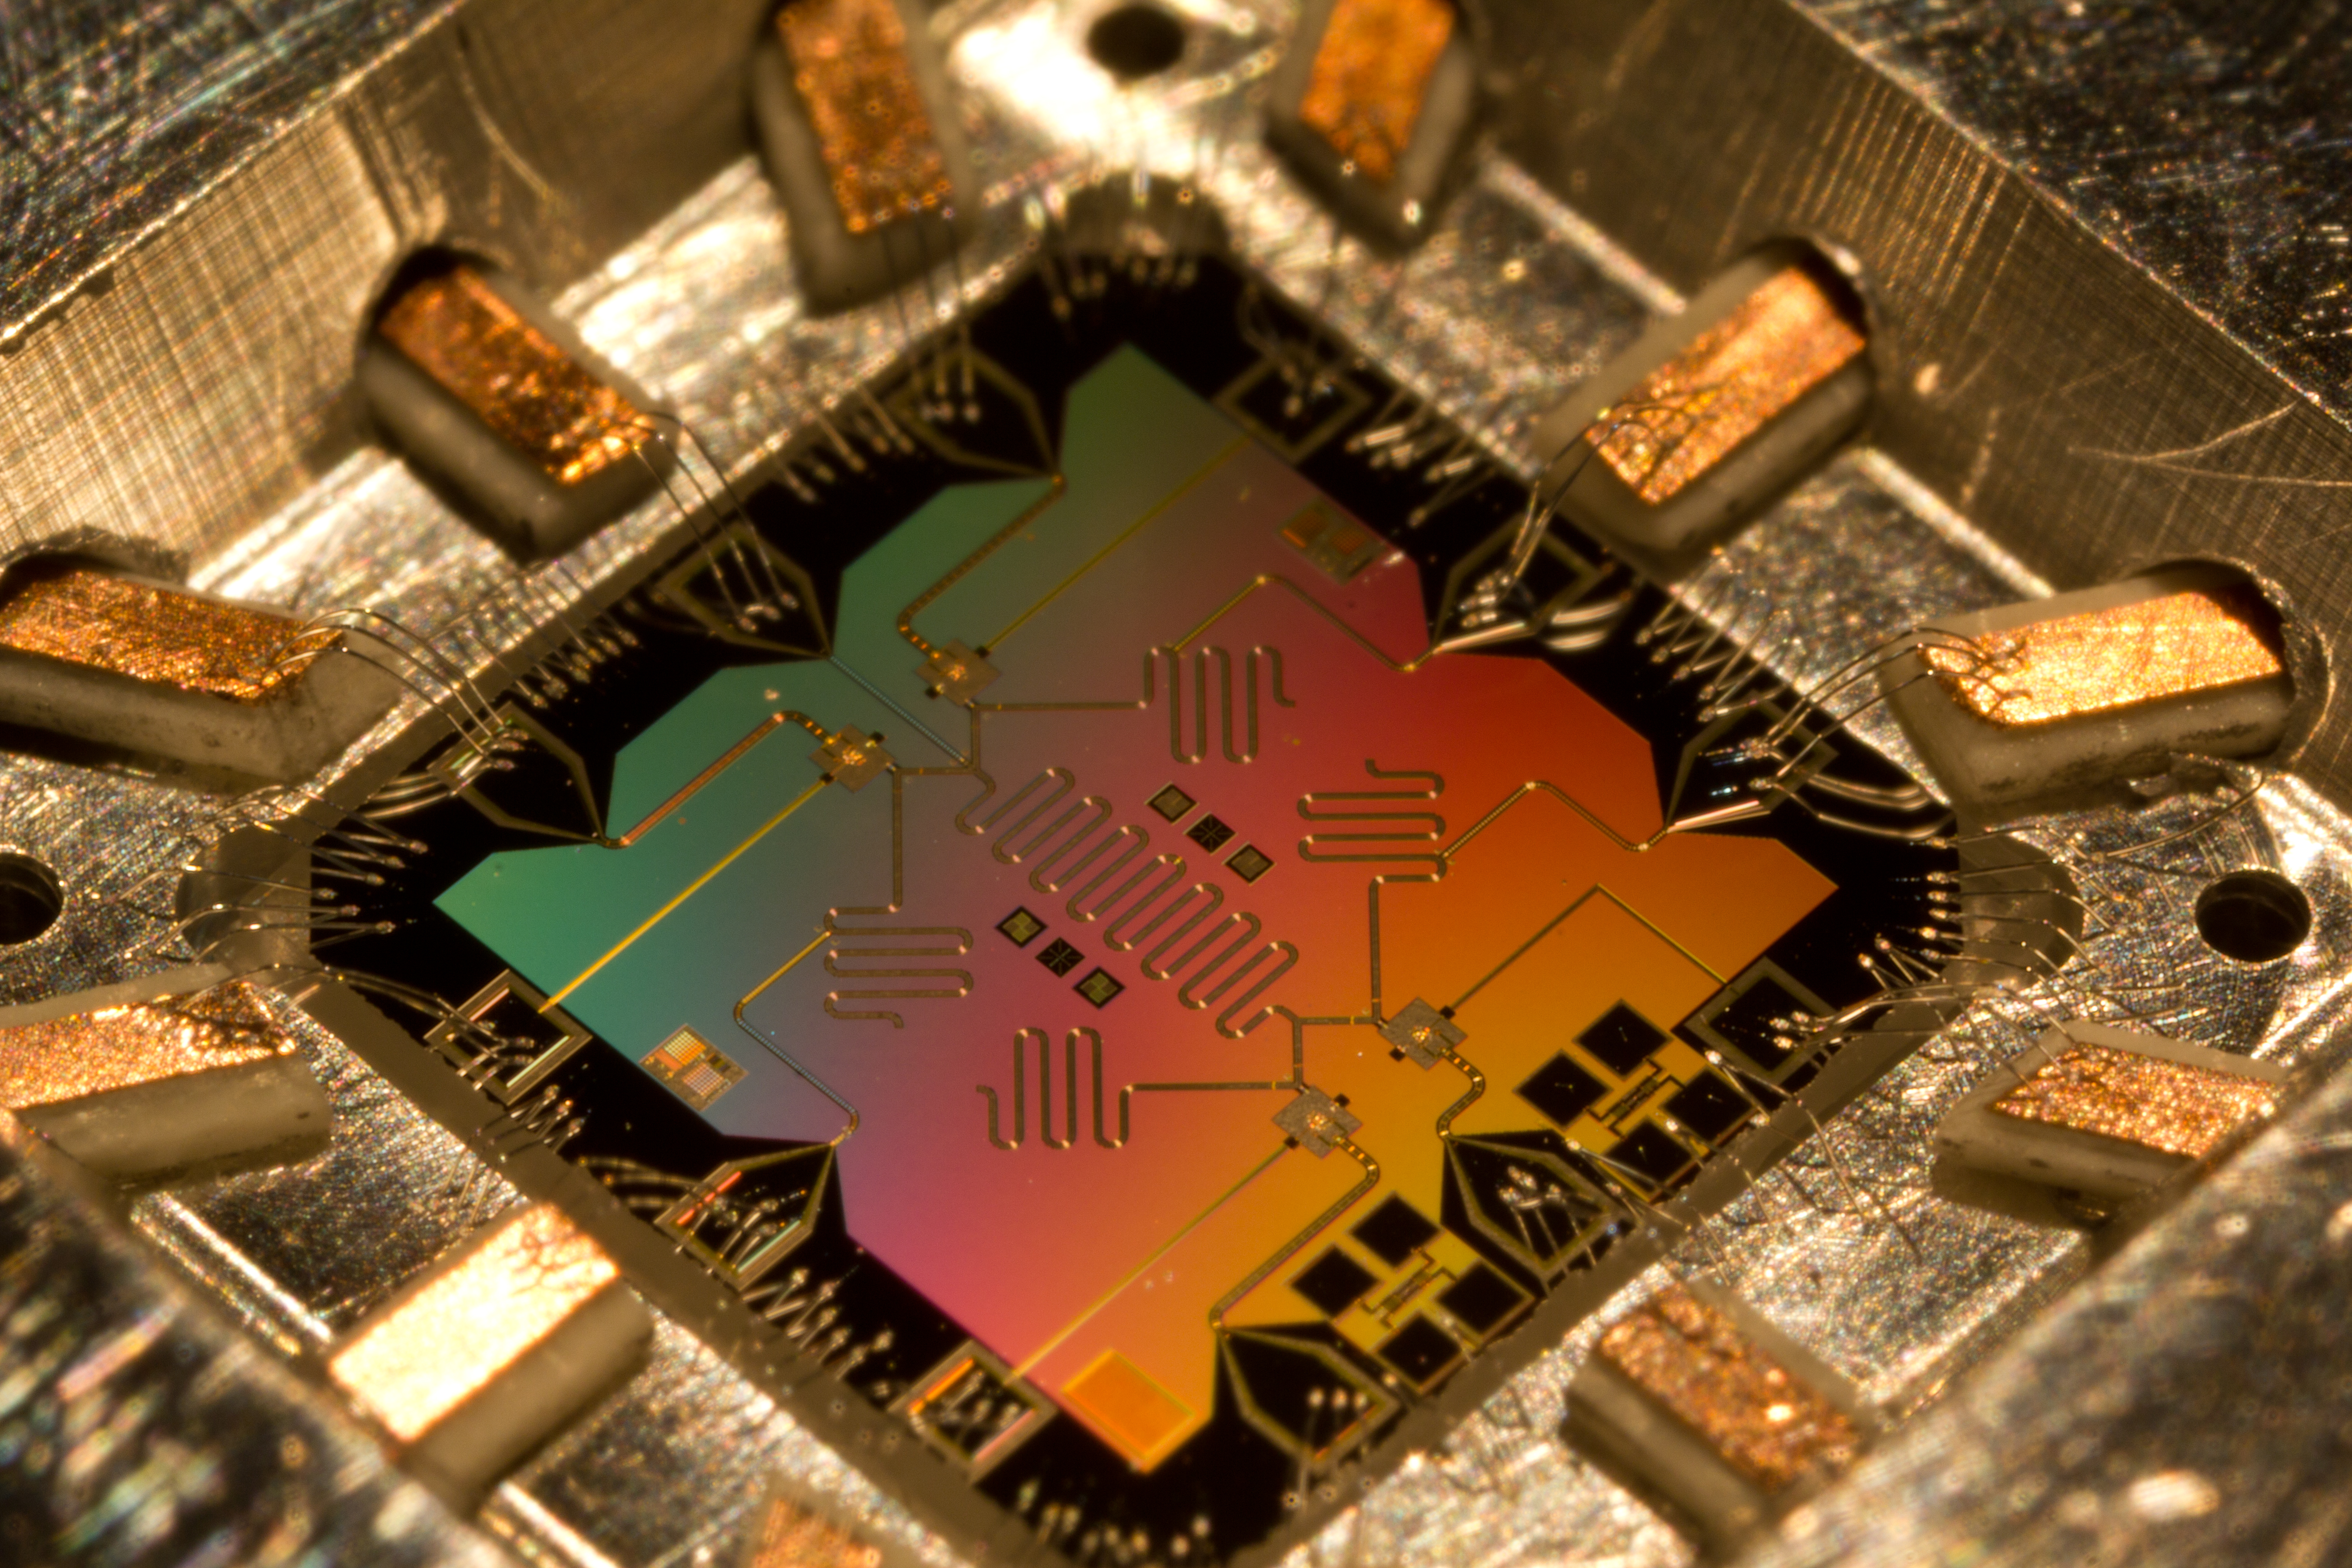
\includegraphics[width=0.6\textwidth]{figures/impl/superconductingchip.jpg}
    \caption{A superconducting chip which contains 2 qubits \cite{supercondpic} \textit{photo by Erik Lucero} \footnotemark}
    \label{fig:superconducting}
\end{figure}

\footnotetext{\url{http://web.physics.ucsb.edu/~martinisgroup/}} 
%%%%%%%%%%%%%%%%%%%%%%%%%%%%%%%%%%%%%%%%%%%%
\subsection{Linear optical quantum computing}

Linear optical quantum computing uses photons and waveguides (commonly referred to as modes) as the qubit. Using light for information processing seems like a natural choice as it is the fastest thing in the universe. Unlike trapped ions and superconducting qubits where their main problem is stopping the qubits interacting with the environment, photons interact very weakly with their environment. This is a positive as we then only have to worry about losing the photons rather than it decohering to a classical object. However, it also means that the two-qubit entangling gates are difficult to perform as photons not only interact weakly with the environment but also do not interact with each other.

Gates are currently performed using electrical heaters which heat locally a small section of the waveguide which in turn changes the phase of the photon\footnote{You can think of the phase of the photon in the same way as the phase of the electric field}. \autoref{fig:loqc} is a fully re-configurable 3 qubit integrated optical chip meaning it can perform any 3 qubit operation. The calculation is performed by using the electrically controlled phase-shifters and interference between the photons to change the probability distribution of which waveguides the photons exit the chip from. The answer to the computation is given by the which waveguides the photons exit.

\begin{figure}[H]
    \centering
    \includegraphics[width=0.7\textwidth]{figures/impl/rekkchip.png}
    \caption{Caption \cite{carolan2015universal}}
    \label{fig:loqc}
\end{figure}

%%%%%%%%%%%%%%%%%%%%%%%%%%%%%%%%%%%%%%%%%%%%
\begin{comment}
\subsection{Error Correction}

Full fault tolerance is beyond the scope of this guide however we will briefly discuss error correction. The basic idea of error correction is to use redundancy to counteract errors. Increasing the resources devoted to storing the logical information should in principle make the computer more resilient to errors.
\end{comment}

%%%%%%%%%%%%%%%%%%%%%%%%%%%%%%%%%%%%%%%%%%%%%%%%%%%%%%%%%%%%%%%%%%%%%%%%%%%%

%%%%%%%%%%%%%%%%%%%%%%%%%%%%%%%%%%%%%%%%%%%%%%%
\section{Physical gate-sets and connectivity restrictions}

Irrespective of the physical platform used to build the quantum computer we can describe the device \footnote{Assuming it is perfect and error-free} with just the gate-set and the connectivity of the device. For example the different platforms above will naturally have access to different gates. In the linear optical platform it turns out to be much easier to perform a Z gate than an X gate. Whereas we could imagine a different system where the opposite is true.

Connectivity describes which qubits are able to interact with each other\footnote{There isn't really an analogy with digital computing as the architectures are so complex we don't worry about which memory addresses are connected to each other, this is the job of the linker}. Ideally to have the most flexible and re-configurable quantum computer we would like to have full connectivity meaning all qubits are able to interact with every other. There are a number of physical implementation reasons why having many qubits connected is hard but we will not cover them here. Instead we highlight the following important fact, for a device to be universal only nearest neighbour connections are needed \autoref{fig:fullconnectivity}. Connectivity is illustrated in \autoref{fig:connectivity}. Currently, none of the devices built have achieved complete nearest-neighbour connectivity. A more likely connectivity is depicted in \autoref{fig:partialconnectivity}. This is due to imperfect fabrication of the devices.

\begin{figure}[H]
    \centering
\begin{subfigure}[h]{0.49\textwidth}
    \centering
    \includegraphics[width=\textwidth]{figures/impl/nearestneighbourcon.png}
    \caption{Full lattice type nearest-neighbour connected qubits}
    \label{fig:fullconnectivity}
\end{subfigure}
~
\begin{subfigure}[h]{0.49\textwidth}
    \centering
    \includegraphics[width=\textwidth]{figures/impl/partialnearestneighbourcon.png}
    \caption{Partially connected qubits}
    \label{fig:partialconnectivity}
\end{subfigure}
\caption{An abstraction of 8 qubit device where the lines illustrate 'connections' between qubits.}
\label{fig:connectivity}
\end{figure}

In the same way that different platforms may be suited to different gate-sets, they may also be suited to different connectivities. For example, the trapped ion platform naturally has nearest neighbour connectivity as a direct result of the tiling scheme. Compare this to LOQC or superconducting qubits where there is no intuitive design for high connectivity due to the restriction that each qubit must be connected to control electronics. Therefore, as the connectivity scales up, so does the density of control lines required, presenting serious electrical engineering challenges.

\subsubsection{Equivalence between different platforms}

Given this information we would like to be able to run a quantum program on any of the equivalent quantum devices (e.g. with the same gate-sets and connectivity). 

We can make a list of possible scenarios for different implementations of two quantum computers:
\begin{table}[h]
    \centering
    \begin{tabulary}{\textwidth}{|c|c||L|}
        \hline
        Gate-set & Connectivity & Fix  \\ \hline  
        %
        Same & Same &  Depends on what the language you have chosen to use returns, easy if both devices use the same quantum Assembly language \footnotemark  \\ \hline
        %
        Same & Different & Use a linker to remap the qubits on the devices \\ \hline
        %
        Different & Same & Use a compiler to perform gate synthesis \\ \hline
        %
        Different & Different & What classical digital compilers and linkers do \\ \hline 
    \end{tabulary}
    \caption{Required software features to convert between different quantum devices}
    \label{tab:gatesandconnectivity}
\end{table}
\footnotetext{We use Assembly here to denote the lowest level language which consists of listing instructions and which qubits the instructions act on}

%%%%%%%%%%%%%%%%%%%%%%%%%%%%%%%%%%%%%%%%%%%%%%%%%%%%

\subsection{Minimal quantum program examples}

We have chosen a minimal program which uses only classical physics, we take the binary representation of the letter 'Q' \footnote{There is nothing special about Q other than the unwritten rule of including q's when naming anything quantum related} and write the value to 8 qubits which represent a qubyte. We then measure the qubits to recover the string. Even for this simple example program we can see some differences between what goes on behind the scenes when using the built in compilers\footnote{A better description would be linker but we will get to that} and we comment on the quantum instruction set languages used. 

Like the other quantum programs above the majority of the quantum hello world program, \autoref{code:quantumhelloworldpyquil} is classical control. A small part of the algorithm uses the quantum computer. This example is novel in that there are no quantum effects used here, however it is more to illustrate the current progress of existing devices. A nice feature we have access to in the quantum case is that we can use either the bit value or phase to store information, instead of X gates an equivalent program could be written which uses H and Z gates.

\autoref{code:quantumhelloworldpyquil} shows the python input to the quantum library which passes in a bit string, the quantum simulator (or processor) is then run for each byte in the bitstring as this only requires 8 qubits. The results of each computation (measurement results) are stored in a python list and then when all of the bytes have been run on the quantum processor the bitstring is translated back into ASCII and printed using python.

We are using this example to show that quantum computers are able to do tasks that classical computers can do, a requirement if we are ever to think of building fully quantum machines (not using the co-processor model).

Even for this simple example there are a number of interesting features that all of the libraries discussed here feature:
\begin{itemize}
    \item The majority of the algorithm is classical classical control 
    \item The simulation has to be run many times to build up a an output distribution
    \item We are currently very limited by existing devices
\end{itemize}

%%%%%%%%%%%%%%%%%%%%%%%%%%%%%%%%%%%%%%%%%%%%%%%%%%%%%%%%%
\subsubsection{Translating pyQuil to quantum hardware}

To use pyQuil on a quantum processor, the source code needs to be be translated into Quil (Quantum Instruction Language) which lists the gates which must be applied to the qubits in the processor. Acts as an intermediate step between pyQuil and the actual instructions that will go to the quantum computer. The Quil compiler \footnote{\url{http://docs.rigetti.com/en/stable/compiler.html}}\footnote{We wouldn't strictly call this a compiler in the usual sense} restricts the quantum gates to the quantum devices gate-set and looks at the connectivity of the machine to make sure (2-qubit) control gates are acting on qubits that are physically connected. 

We will give an example of the compilation process in pyQuil using a simple Hello World program, shown below in \autoref{code:quantumhelloworldpyquil}. We specify the 8 qubit Agave device architecture which then maps the Quill code written to the device gate-set and connectivity. 

%%%%%%%%%%%%%%%%%%%%%%%%%%%%%%%%%%%%%%%%%%%%%%%%%%%%%%%%%%%%%%
\subsubsection{Translating QISKIT (Quantum Information Science KIT) to hardware}

The Qiskit library has to translate the python code into IBM's Open quantum assembly (OQASM) to be run on their devices. IBM has multiple quantum devices (3, 4, 5 and 16 qubit devices) that you can run quantum programs on. Qiskit also comes with a local simulator, similar to pyQuil which can simulate up to 32 qubits. An API key is needed to access the quantum devices but not the local simulator.

Here we give an example of the Qiskit python library code and the OQASM output \footnote{the user can write QASM embedded in Python and Qiskit will return the program as QASM \footnotemark} \footnotetext{There is no spelling mistake here...}. We tried compiling the OQASM to a device specific arcitecture but couldn't get the program to reduce or simplify the gates.

%%%%%%%%%%%%%%%%%%%%%%%%%%%%%%%%%%%%%%%%%%%%%%%%%%%%%%%%%
\subsubsection{Translating Project Q to hardware}

ProjectQ is one of the more flexible quantum programming languages available in terms of the types of operations, compilers and back-ends that are available. Many of the typical gates that are used in quantum algorithms are already built in, and user defined gates that are either just matrices or based on mathematical operations are relatively simple to implement. 

Project Q is also the only library discussed here that comes with a local simulator. You can also a specify machine architecture for IBM devices using the IBM compatible compiler \cite{zulehner2018efficient} which will compile the project Q code into the gate-set and connectivity of the specified machine.
%%%%%%%%%%%%%%%%%%%%%%%%%%%%%%%%%%%%%%%%%%%%%%%%%%%%%%%%%
\subsubsection{Translating Q\# to hardware}

It is not currently possible to convert code written in Q\# to hardware. This is because there is only a simulator and no way to obtain the list of gates that are being simulated. We have therefore not included a minimal example of compiling Q\# code to hardware level instructions.

Q\# does however support a resource counter which estimates the resources required to run the quantum program on hardware. We give a minimimal example showing 

%%%%%%%%%%%%%%%%%%%%%%%%%%%%%%%%%%%%%%%%%%%%%%%%%%%%%%%%%
% code
\noindent \begin{minipage}[t]{0.45\textwidth}
\begin{listing}[H]
   \inputminted{python}{code/asm/pyquil_helloworld.txt} 
    \caption{Pyquil Hello Q program}
\end{listing}
\end{minipage} \hfill 
\begin{minipage}[t]{0.45\textwidth}
\begin{listing}[H]
   \inputminted[lastline=15]{python}{code/asm/pyquil_helloworld_output.txt}
   \caption{Quil code from pyQuil code}
\end{listing}
\begin{listing}[H]
   \inputminted[firstline=17, lastline=37]{python}{code/asm/pyquil_helloworld_output.txt}
   \caption{Compiled code using the 8 qubit AGAVE devce architecture}
\end{listing}
\end{minipage}

%%%%%%%%%%%%%%%%%%%%%%%%%%%%%%%%%%%%%%%%%%%%%%%%%%%%%%%%%%%%%%

%%%%%%%%%%%%%%%%%%%%%%%%%%%%%%%%%%%%%%%%%%%%%%%%%%%%%%%%%%%%%%
% code
\noindent \begin{minipage}[t]{0.55\textwidth}
\begin{listing}[H]
   \inputminted{python}{code/asm/text/progqiskithello.txt}
   \caption{Qiskit hello world}
\end{listing}
\end{minipage} \hfill 
\begin{minipage}[t]{0.3\textwidth}
\begin{listing}[H]
   \inputminted[firstline=2,lastline=18]{python}{code/asm/qiskit_helloworld.output.txt}
   \caption{OQASM for the qiskit hello world program}
\end{listing}
\begin{listing}[H]
   \inputminted[firstline=21]{python}{code/asm/qiskit_helloworld.output.txt}
   \caption{OQASM for the qiskit hello world program}
\end{listing}
\end{minipage}


\begin{comment}
\url{https://github.com/Qiskit/qiskit-terra}
\url{https://github.com/Qiskit/openqasm/tree/master/examples}
\url{https://github.com/Qiskit/qiskit-tutorial/blob/master/reference/algorithms/grover_algorithm.ipynb}
\url{https://github.com/Qiskit/qiskit-tutorial/blob/master/appendix/advanced_qiskit/compiling_and_running.ipynb}
the qiskit backends are here \url{https://github.com/Qiskit/qiskit-backend-information/tree/master/backends}
QASM documentation here \url{https://github.com/Qiskit/openqasm/blob/master/spec/qasm2.rst}
The Qiskit compiler \url{https://developer.ibm.com/code/2017/05/17/developers-guide-to-quantum-qiskit-sdk/}
\end{comment}
%%%%%%%%%%%%%%%%%%%%%%%%%%%%%%%%%%%%%%%%%%%%%%%%%%%%%%%%%%%%%%

%%%%%%%%%%%%%%%%%%%%%%%%%%%%%%%%%%%%%%%%%%%%%%%%%%%%%%%%%%%%%%
% code
\noindent \begin{minipage}[t]{0.6\textwidth}
\inputminted{python}{code/asm/text/progprojqhello.txt}
\end{minipage} \hfill 
\begin{minipage}[t]{0.37\textwidth}
\inputminted[lastline=29]{python}{code/asm/projqout.txt}
\inputminted[firstline=31]{python}{code/asm/projqout.txt}
\end{minipage}

\subsubsection{Q\# example}

That's right. There is no example.

%%%%%%%%%%%%%%%%%%%%%%%%%%%%%%%%%%%%%%%%%%%%%%%%%%%%%%%%%%%%%%
\subsection{Summary}

We now compare some of the implementation dependent features of the languages and give a comparison between them.
%%%%%%%%%%%%%%%%%%%%%%%%%%%%%%%%%%%%%%%%%%%%%%%%%%%%%%%%5
\subsubsection{Qubit management}

The pyQuil qubit management is dynamic, qubits are allocated dynamically which does not require the users input. The qiskit library is heavily based on using quantum circuits. You specify quantum and classical registers and ancilla qubits. Project Q also requires the user to manually allocate qubits and the QASM resembles dynamically allocated qubits with allocate and deallocate at the start and end of the instruction set. 

%%%%%%%%%%%%%%%%%%%%%%%%%%%%%%%%%%%%%%%%%%%%%%%%%%%%%%%%5
\subsubsection{Compilers/Gate simplification}

All of the libraries have access to the standard gate set in their python environments\footnote{X,Y,Z,H,Phase gates and arbitrary rotations}. 

In pyQuil the user can also use the \texttt{defgate()} method to define their own gate either in terms of compositions of existing gates or by specifying a matrix representation of the gate. Qiskit also can define gates. Project Q has the option to define gates?

The pyQuil compiler takes one of Rigetti's quantum devices as an argument and compiles their Quill QASM into device specific gate-set and remaps the qubits to match the connectivity of the machine.

IBM has no working compiler\footnote{there is a compiler but it does nothing, specify x only and the program crashes, specify x and H and the program uses Z. U(x,y,z)($\theta$).} but we can return the Open QASM (IBM's Quantum Assembly format), 

The Project Q compiler is designed to have a modular structure, so the user can pick and choose the level of optimisation required. It works quite well although you have to manually specify the available gate-set you have access to and the connectivity of the machine. They are working on adding in backend support for the IBM quantum devices.


%%%%%%%%%%%%%%%%%%%%%%%%%%%%%%%%%%%%%%%%%%%%%%%%%%%%%%%%5
\begin{comment}
\subsubsection{Resource counters}

All of the software packages support resource counting of some sort.

\end{comment}
%%%%%%%%%%%%%%%%%%%%%%%%%%%%%%%%%%%%%%%%%%%%%%%%%%%%%%%%5
\subsubsection{Backends}

Rigetti then offers a remote Quantum Virtual Machine (QVM) which runs simulations of up to 26 qubits requiring an API key to use. They do not provide a local simulator which runs on a personal computer. IBM do provide a local simulator and access to their devices and remote simulator require and API key. Project Q comes with a local simulator, written in c++ and is built on your machine on install using python wrappers.

The project Q simulator is best of the local simulators however currently there is no way to compile project Q code into IBM's OASM to run on IBM's machines or compile to Quil to run on Rigetti's machines. Although IBM and Project Q existed as part of the same project \footnote{see git change-log} we are unsure of when the project Q to IBM backend will be implemented. 

One slightly annoying feature of pyQuil the software package is the lack of local quantum simulator. This can cause problems when trying to execute large programs as we often found the connection timed out before the program finished. 

%%%%%%%%%%%%%%%%%%%%%%%%%%%%%%%%%%%%%%%%%%%%%%%%%%%%%%%%5
\subsubsection{Device mappings}

Rigetti's Quil compiler takes a dictionary of one of their devices which then creates a map of the positions of the qubits and the connectivity of the machine. 

QISKits' \texttt{get remote backends} method doesn't return any valid devices to compile to, when using one of their device names an error saying the device is not valid is produced. It may be possible to manually add device mappings but even then the \textit{compiler} didn't compile to the given gate-set or it would produce an error for some gate-sets.

Project Q lets you specify the connectivity using a Python dictionary and gate-set by importing the gates you want/have access to. The compiler works quite well.

\section{Comparing classical and quantum compilers}

In the previous section we showed how quantum compilers work. They take source code (for example pyQuil) and turn it into a low level set of operations (for example Quil) which can be executed on a quantum device or simulator. The compiler performs certain optimisation operations (for example simplifying $HZH$ to $X$) but does not otherwise substantially modify the source code. 

Here we show, by way of comparison, the compilation steps that turn a classical program (Hello world, written in C) into an executable file. Our aim is to show that there are many more steps in the process, including optimisation and linking, which are not really present in the quantum case. We will discuss in detail what each of these steps are, why they are necessary and how they occur in a classical computer. We will then speculate on which of how quantum compilation may eventually develop as the complexity of quantum programs increases.

\begin{comment}

Quantum compilers have a range of meaning depending on who you ask, we hope to clarify some of the common misconceptions\footnote{The use of compiler is abused in all of the quantum libraries discussed here} in the following section. 


We give an example of a simple Assembly program. Much like the the \textit{quantum languages} covered in this guide, assembly code is contains a list of operations, drawn from an instruction set, that the computer should perform. 


Unlike interpreted languages, assembly needs to first be assembled and then linked. Assembling is the process which turns assembly language into object code -- this is a small block of machine code which cannot be directly executed because none of its contents (variables etc.) have memory addresses yet. The linker takes an object file and produces an executable file where all the addresses are properly defined. The linker can also process multiple object files, producing a single executable file. The linker provides flexibility in allocating the resources needed to run a program. Below we give some examples illustrating the purposes of compilers and linking.

We now include a \textit{Hello world!} program, even in this simple program case we can see that the linker is important.
\end{comment}



%%%%%%%%%%%%%%%%%%%%%%%%%%%%%%%%%%%%%%%%%%%%%%%%%%%%%%%%%
\subsection{Compile, Assemble, link, execute}

As shown in \autoref{fig:compileasslinkrun}, there are three steps which turn a classical compiled language such as C into a program which can be executed on a classical computer. We will demonstrate this process in the case of a simple \textit{Hello World!} program written in C. The program prints the string "Hello World!" and exits, returning 0 to the operating system. This is shown in \autoref{code:c_helloworld}.

\noindent \begin{minipage}{0.65\textwidth}
% c code
\begin{listing}[H]
   \inputminted{c}{code/asm/c_helloworld.txt}
   \caption{Hello world! in C}
   \label{code:c_helloworld}
\end{listing}

The compiler takes this C source file as an input, and outputs the assembly language file shown in \autoref{code:asm_helloworld}. The assembly file looks very different to the original source code, because it contains instructions like movl and call. These instructions performs a basic operations such as moving data around or calling sub-routines. There is normally a large degree of optimisation that goes into this step, because the language constructs in C do not map directly to instructions in assembly language. 

% asm code
\begin{listing}[H]
   \inputminted[firstline=8, lastline=22]{gas}{code/asm/c_helloworld.x86_64.txt}
   \caption{Assembly file after compiling}
   \label{code:asm_helloworld}
\end{listing}
\end{minipage} \hfill
%
\begin{minipage}{0.3\textwidth}
    \centering
    \includegraphics[width=1.1\textwidth]{figures/impl/compileassemblelinkrun.png}
    \captionof{figure}{Compile, assemble, linking and running structure for running a program}
    \label{fig:compileasslinkrun}
\end{minipage}

The assembler then turns the assembly language file into an object file, shown in the left hand part of \autoref{code:obj_helloworld}. This is quite a simple step -- it involves replacing all the instructions with strings of numbers called machine code which is readable by the target computer. The right hand column shows the instructions corresponding to the codes on the left. The critical feature of the object file is the lack of addresses. For example lines 3 and 4 contain placeholders \$0x0 and e. These addresses are resolved by the linker, which assigns memory to all the variables. The linked file is shown in \autoref{code:exe_helloworld}. Notice how the program itself has also been assigned a memory location -- line 1 shows that the first instruction is at address 400526. In larger programs, each source file has its own object file. The linker combines all these files together to produce an executable file which can be run on the target computer.

% object filoe
\begin{listing}[H]
   \inputminted[firstline=40, lastline=46]{gas}{code/asm/c_helloworld.x86_64obj.txt}
   \caption{Object file before linking}
   \label{code:obj_helloworld}
\end{listing}

\begin{listing}
   \inputminted[firstline=137, lastline=143]{gas}{code/asm/c_helloworld.x86_64obj.txt}
   \caption{Executable file after linking}
   \label{code:exe_helloworld}
\end{listing}

%%%%%%%%%%%%%%%%%%%%%%%%%%%%%%%%%%%%%%%%%% tikz
\begin{comment}
\tikzstyle{every picture}+=[remember %picture,inner xsep=0,inner ysep=0.25ex]

% c prog
\begin{code}
\inputminted[]{c}{code/asm/c_helloworld.txt}
\captionof{listing}{Hello world! in C 
\tikz[remember picture] \node [] (a){ };}
\label{code:c_helloworld}
\end{code}


\begin{tikzpicture}[remember picture, overlay]
\draw[->, line width=1mm] (a.south) -- %++(0,-2ex) node[anchor=north] {Compiler} -| %(b.north) ;  
\end{tikzpicture}

%% compiled c prog
\begin{code}
\tikz[remember picture] \node [] (b) {};
\inputminted[firstline=8,lastline=22]{gas}{code/asm/c_helloworld.x86_64.txt}
\captionof{listing}{Assembly code of Hello world! in C 
\tikz[remember picture] \node [] (c) {};}
\end{code}

\begin{tikzpicture}[remember picture, overlay] 
\draw[->, line width=1mm] (c.south) -- %++(0,-1.5ex) -| (d.north) ;
\end{tikzpicture}

%% assembled c prog
\begin{code} 
\tikz[remember picture] \node [] (d) {};
\inputminted[firstline=37,lastline=46]{objdump}{code/asm/c_helloworld.x86_64obj.txt}
\captionof{listing}{Object dump of the Hello world assembled object file 
\tikz[remember picture] \node [] (e) {};}
\end{code}

\begin{tikzpicture}[remember picture, overlay]
\draw[->, line width=1mm] (e.south) -- ++(0,-1.5ex) -| (f.north) ;
\end{tikzpicture}

% linked c prog
\begin{code} 
\tikz[remember picture] \node [] (f) {};
\inputminted[firstline=60,lastline=74]{objdump}{code/asm/c_helloworld.x86_64obj.txt}
\captionof{listing}{Object dump of the executable program after compiling, assembling and linking, we have truncated the code early here.
\tikz[remember picture] \node [] (g) {};}
\end{code}


%%%%%%%%%%%%%%%%%%%%%%%%%%%%%%%%%%%%%%%%%%%%%%%%
\begin{tikzpicture}[overlay]
    % Bend above text line
    %\draw[-latex] (node2.north) to[bend right] (node1.north);
    % Bend below text line
    %\draw[-latex] (node2.south) to[bend left] (node1.south);
    % Angled
    \draw[-latex] (node5.south) -- ++(0,-1.5ex) -| (node6.north);
\end{tikzpicture}
\end{comment}
%%%%%%%%%%%%%%%%%%%%%%%%%%%%%%%%%%%%%%%%%%%%%%%%%

%%%%%%%%%%%%%%%%%%%%%%%%%%%%%%%%%%%%%%%%%%%%%%%%%%%%%%%%%%%%%%%%%%%%
\subsection{Quantum compilation}

\begin{wrapfigure}{r}{0.4\textwidth}
    \centering
    \includegraphics[width=0.45\textwidth]{figures/impl/quantumcompilefixrun.png}
    \caption{quantum instruction set flow}
    \label{fig:quantumcompile}
    \vspace{-30pt}
\end{wrapfigure}

Quil, OQASM and Project Q's quantum assembly have laid the ground work for building a quantum programming language. Although we suspect it will be some time before we get a full quantum language and not domain specific embedded languages, the work on quantum instruction sets has a long way to go. 

The main feature we would like to highlight is that because Assembly is such a low-level language, the program is doesn't need to be compiled, the action of the assembler and linker is to rename the human readable code into machine code and allocate memory for the program. This is exactly the same as the quantum libraries discussed here \footnote{see the cloud based section, the python code and \textit{compiled} code are relabelings of each other}.

quantum computers have linkers at the moment. what a compiler is and should be for quantum computer. The assembler process which assigns temporary addresses to parts of the object file is similar to a lot of the resource counting steps that the current quantum libraries and languages have.

%%%%%%%%%%%%%%%%%%%%%%%%%%%%%%%%%%%%%%%%%%%%%%%%%%%%%%%%%%%%%%%%%%%%%%%%

%\begin{verbatim}
%% TODO IN A LATER VERSION. :(

%%%%%%%%%%%%%%%%%%%%%%%%%%%%%%%%%%%%%%%%%%%%%%%%%%%%%%%%%%%%%%%%%%%%%%%%
%                                                                      %
%%%%%%%%%%%%%%%%% RIP FORTRAN YOU MAGNIFICENT BASTARD %%%%%%%%%%%%%%%%%%
%                                                                      %
%%%%%%%%%%%%%%%%%%%%%%%%%%%%%%%%%%%%%%%%%%%%%%%%%%%%%%%%%%%%%%%%%%%%%%%%

%%%%%%  %%%%%%%%    %%%%%%   %%%%%%%    %%%%%%         %       %       %
%       %      %    %     %     %       %     %       % %      % %     %
%%%%%   %      %    %   %       %       %   %        % % %     %   %   %
%       %      %    %    %      %       %    %      %     %    %    %  %
%       %%%%%%%%    %     %     %       %     %    %       %   %     % %

% this took longer than you'd think
%\end{verbatim}


%
%%%%%%%%%%%%%%%%%%%%%%%%%%%%%%%%% END OF USEFUL CONTENT
%

\begin{comment}

\subsubsection{Rigetti's Forest}

We will now discuss in detail the structure of what happens when the code examples above are run. For Rigetti \url{http://docs.rigetti.com/en/stable/compiler.html#region-specific-compiler-features-through-pragma}

The structure of Rigetti's quantum programming environment is as follows:
\begin{itemize}
    \item \textbf{Forest} - Rigetti's entire quantum programming toolkit. Overall the Forest documentation is very good\footnote{\url{docs.rigetti.com/en/stable/}}
    \item \textbf{pyQuil} - Open source Python library. The user writes their code in pyQuil\footnote{There is a kind of standard library for pyQuil called Grove} and this gets translated to Quil .
    \item \textbf{Quil} – Quantum Instruction Language which is assembly-like as it lists the gates to apply. Acts as an intermediate step between pyQuil and the actual instructions that will go to the quantum computer.
    \item \textbf{Execution} Rigetti has a Quantum Virtual Machine \textbf{QVM} which runs simulations of up to 26 qubits - an API key is required to access this. (They do not provide a local simulator.) They also have Quantum Processing Units \textbf{QPUs}, which are actual chips with physical qubits which requires special access.
\end{itemize}

%%%%%%%%%%%%%%%%%%%%%%%%%%%%%%%%%%%%%%%%%%%%%%%%%%%%%
\subsubsection{IBM's QISKIT (Quantum Information Science KIT)}


The current state of IBM's stack, from top to bottom consists of the following elements:

\begin{itemize}
    \item \textbf{QISKit} - IBM's open source quantum library for usage in the high level language Python \footnote{There is a standard library for algorithms called ACQUA}.
    \item \textbf{OpenQASM} – IBM's low-level Quantum Assembly Language which interprets commands and functions from QISKit and translates them into microwave pulses for use on the physical architecture (superconducting qubits). Acts as an intermediate step between QISKit and the actual instructions that will go to the quantum computer.
    \item \textbf{Execution} \textbf{QPU} - IBM has multiple physical architectures for running quantum algorithms. These include 3, 4, 5 and 16 qubit devices accessible via an API provided when you create an account with the IBM Experience, and larger 20 qubit devices that are available via membership to the IMB Q Network (hubs, partner institutions etc). \textbf{Q QASM Simulator} - IBM's Quantum Virtual Machine which runs simulations of up to 32 qubits, an API key is required to access this.
\end{itemize}

The devices used to perform the simulation and computation are based on a superconducting charge qubit implementation, which can be found described in more detail in \autoref{chpt:implementations}. 

Open QASM is their quantum assmbely language, Qiskit is the Quantum Information Science Kit which is a python library where the user can write QASM and Qiskit will translate it into QASM \footnote{somehow but I haven't figured it out yet...}. 


%%%%%%%%%%%%%%%%%%%%%%%%%%%%%%%%%%%%%%%%%%%%%%%%%%%%%%%%%
\subsubsection{Project Q}

\begin{figure}[h]
    \centering
    \includegraphics[width=\textwidth]{projectq_structure.PNG}
    \caption{Structure of ProjectQ. Taken from \cite{projectq2018}, will make own diagram and possibly simplify.}
\end{figure}

ProjectQ is one of the more flexible quantum programming languages available in terms of the types of operations, compilers and back-ends that are available. Many of the typical gates that are used in quantum algorithms are already built in, and user defined gates that are either just matrices or based on mathematical operations are relatively simple to implement. 

\begin{itemize}
    \item Python library
    \item Local simulator
    \item Can specify machine architecture for IBM devices
\end{itemize}
%%%%%%%%%%%%%%%%%%%%%%%%%%%%%%%%%%%%%%%%%%%%%%%%%%%%%%%%%

%%%%%%%%%%%%%%%%%%%%%%%%%%%%%%%%%%%%%%%%%%%%%%%%%%%%%%


\end{comment}


\begin{comment}
% code
% left side
\begin{minipage}[t]{0.4\textwidth}
\begin{code}
\captionof{listing}{Hello world! in C}
\inputminted[]{c}{code/asm/c_helloworld.txt} 
\end{code}
\end{minipage} \hfill 
% right side
\begin{minipage}[t]{0.6\textwidth}
\begin{code}
\captionof{listing}{Assembly code of Hello world! in C}
\inputminted[]{gas}{code/asm/c_helloworld.x86_64.txt}
\end{code}
\end{minipage}

The compiler has completely changed the C function into Assembly code. 

The next step is to assemble the assembly code into an object file,

% code
%{\renewcommand\fcolorbox[4][]{\textcolor{cyan}{\strut#4}}
% left side
%\begin{minipage}[t]{0.49\textwidth}
\begin{code}
\inputminted[firstline=32, lastline=51]{objdump}{code/asm/c_helloworld.x86_64obj.txt} 
\captionof{listing}{Object dump of the Hello world assembly file}
\end{code}
%\end{minipage} \hfill 
% right side
%\begin{minipage}[t]{0.49\textwidth}

after assembling the file we now have to link the file to assign actual memory locations.
\begin{code}
\inputminted[firstline=55, lastline=74]{objdump}{code/asm/c_helloworld.x86_64obj.txt}
\captionof{listing}{Object dump of the executable program after compiling, assembling and linking, we have truncated the code early here.}
\end{code}
\end{comment}
%\end{minipage}
%}


%FORTRAN and C are both functional languages and follow a clear structure

\begin{comment}
\subsubsection{x86 Assembly}
% program
%\lstinputlisting[language=Asmx86, firstline=1, lastline=25, caption={Hello world program}, label={code:helloworldasm}]{code/asm/printobj.txt}

\begin{code}
\inputminted[firstline=2, lastline=25]{gas}{code/asm/printobj.txt}
\captionof{listing}{Hellow world program in x86 asm}
\label={code:helloworldasm}
\end{code}
The program when run returns the string \textit{Hello World} to the terminal. In order to run the program we must assemble and then link the object file. Assembling the program produces an object file, we can dump the contents of the file and look at what the assembler does to a program,

% assembled
%\lstinputlisting[language=Asmx86, firstline=27 , lastline=48, caption={Hello world assembled}, label={code:assembledhelloworldasm}]{code/asm/printobj.txt}
\begin{code}
\inputminted[firstline=28,lastline=48]{objdump}{code/asm/printobj.txt}
\captionof{listing}{Hello world assembled}
\label={code:assembledhelloworldasm}
\end{code}

\autoref{code:assembledhelloworldasm} is the assembled object dump for the \textit{Hello world} program. The assembler has given temporary memory addresses to the object file. This is similar to a lot of the resource counting steps that the current quantum libraries and languages have. 

In order to produce executable code we have to link the object which assigns it actual memory locations. Linking can be done using the GNU Linker, \textit{ld}. This produces another file which we can view using objectdump to see what the linker has done.

% linked
%\lstinputlisting[language=Asmx86, firstline=51 , lastline=72, caption={Hello world assembled and linked}, label={code:linkedhelloworldasm}]{code/asm/printobj.txt}

\begin{code}
\inputminted[firstline=52, lastline=72]{objdump}{code/asm/printobj.txt}
\captionof{listing}{Hello world assembled and linked}
\label{code:linkedhelloworldasm}
\end{code}

\autoref{code:linkedhelloworldasm} is the linked and assembled code for the \textit{Hello world} program Now the memory locations have been assigned to the code.

\autoref{code:assembledhelloworldasm} is the dump of the assembled object code and \autoref{code:linkedhelloworldasm} is the dump of the assembled and linked object code. 
\end{comment}


%%%%%%%%%%%%%%%%%%%%%%%%%%%%%%%%%%%%%%%%%%%%%%%%%%%%%%%%%%%%%%%%%%%%%%%%

%\begin{verbatim}
%% TODO IN A LATER VERSION. :(

%%%%%%%%%%%%%%%%%%%%%%%%%%%%%%%%%%%%%%%%%%%%%%%%%%%%%%%%%%%%%%%%%%%%%%%%
%                                                                      %
%%%%%%%%%%%%%%%%% RIP FORTRAN YOU MAGNIFICENT BASTARD %%%%%%%%%%%%%%%%%%
%                                                                      %
%%%%%%%%%%%%%%%%%%%%%%%%%%%%%%%%%%%%%%%%%%%%%%%%%%%%%%%%%%%%%%%%%%%%%%%%

%%%%%%  %%%%%%%%    %%%%%%   %%%%%%%    %%%%%%         %       %       %
%       %      %    %     %     %       %     %       % %      % %     %
%%%%%   %      %    %   %       %       %   %        % % %     %   %   %
%       %      %    %    %      %       %    %      %     %    %    %  %
%       %%%%%%%%    %     %     %       %     %    %       %   %     % %

% this took longer than you'd think
%\end{verbatim}


%
%%%%%%%%%%%%%%%%%%%%%%%%%%%%%%%%% END OF USEFUL CONTENT
%